\frame{\section{Stato dell'arte}
\subsection[Parametri]{Parametri della deambulazione}
\frametitle{Parametri della deambulazione}

\begin{columns}
\column[b]{.25\textwidth}
\begin{block}{Modellazione}
\begin{enumerate}
	\item Heel Strike
	\item Foot Flat
	\item Heel Off
	\item Toe Off
\end{enumerate}
\end{block}
\column{.8\textwidth}
\begin{figure}
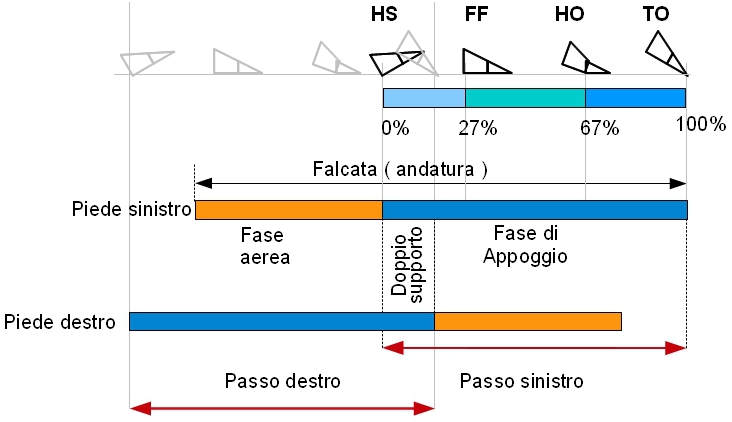
\includegraphics[width=1\textwidth]{imgs/cicloPasso.jpg}\\
\end{figure}

\begin{block}{Valutazione}
\begin{enumerate}
	\item Velocit�: $v\,[m/s]$
	\item Cadenza: $C = num\,passi / s$
\end{enumerate}
\end{block}
\end{columns}
} 


\frame{
\subsection[Letteratura]{Stima dei parametri della deambulazione in letteratura}
\frametitle{Stima dei parametri della deambulazione in letteratura}
\begin{columns}
\column[t]{.5\textwidth}
\begin{block}{Miyazaki (1997) \cite{unrestrained_measurement_stride_length_gyr}}
\textbf{Strumento}: Giroscopio uniassiale \\
\textbf{Posizione}: coscia\\
\textbf{Metodo}: integrazione velocit� angolare
\end{block}
\column[t]{.5\textwidth}
\begin{block}{Aminian et al.(2002) \cite{spatio_temporal_params_gait_gyr}}
\textbf{Strumento}: 2 Giroscopi\\
\textbf{Posizione}: coscia e stinco\\
\textbf{Modello}: modello biomeccanico a pendolo invertito della gamba\\ 
\textbf{Metodo}: basato sulle trasformate \textit{Wavelet}
\end{block}
\end{columns}

\begin{columns}
\column{.5\textwidth}

	\begin{block}{Sabatini et al (2005) \cite{walking_features_from_inertials}}
	\textbf{Strumento}:  1 Giroscopio monoassiale, 2 accelerometri biassiali\\
	\textbf{Posizione}: collo del piede \\
	\textbf{Metodo}: basato su soglie (\textit{threshold-based})
	\end{block}
\column{.5\textwidth}
%	\footnotesize{
%	\begin{table}%
%%	\centering
%	\rowcolors{1}{RoyalBlue!20}{RoyalBlue!5}
%	\begin{tabular}{c|l l}
%	\textbf{E} & \multicolumn{2}{l} {\textbf{regola}}\\
%	%\hline
%	\hline
%	$t_{HS}$ & $ \omega_k \leq 0 $ e $ min_1 \leq  \omega_k$ & $\displaystyle\max_{\forall k}|\widetilde{\omega_k} - \omega_k|$\\
%	%\hline
%	$t_{FF}$ & $|\omega_k|\geq  50$�/s&\\
%	%\hline
%	$t_{HO}$ & $|\omega_k|\geq  50$�/s &\\
%	%\hline
%	$t_{FO}$ & $\omega_k = 0$ & se $\omega$ � diventato positivo \\
%	&\multicolumn{2}{l}{e cresce fino a max.}\\
%	\end{tabular}
%	%\caption{Regole basate sulle soglie (\textit{threshold based}) mediante le quali vengono ricavati gli eventi che delimitano le 4 fasi del cammino \cite{walking_features_from_inertials}.}
%	%\label{tab:regole_threshold_eventi}
%	\end{table}
%	}

\begin{block}{Pfau et al (2008) \cite{stride_segmentation_technique_hmm}}
\textbf{Strumento}:  1 accelerometro triassiale, 1 giroscopio triassiale, un magnetometro\\
\textbf{Posizione}: dorso e torace \\
\textbf{Modello}: HMM per la segmentazione del galoppo\\
\end{block}

\end{columns}
} 

%\frame{
%\frametitle{Materiali e Metodi per la stima dei parametri della deambulazione}
%\begin{block}{Aminian et al.(2002) \cite{spatio_temporal_params_gait_gyr}}
%\textbf{Strumento}: 2 Giroscopi\\
%\textbf{Posizione}: coscia e stinco\\
%\textbf{Modello}: modello biomeccanico a pendolo invertito della gamba\\ 
%\textbf{Metodo}: basato sulle trasformate \textit{Wavelet}
%\end{block}
%} 

%\frame{
%\begin{figure}
%\frametitle{Materiali e Metodi per la stima dei parametri della deambulazione}
%\begin{block}{Sabatini et al (2005) \cite{walking_features_from_inertials}}
%\textbf{Strumento}:  1 Giroscopio monoassiale, 2 accelerometri biassiali\\
%\textbf{Posizione}: collo del piede \\
%\textbf{Metodo}: basato su euristiche (\textit{threshold-based})
%\end{block}
%\centering
%\end{figure}
%\begin{table}%
%\centering
%\begin{tabular}{c|l p{4cm}}
%\textbf{Evento} & \multicolumn{2}{c} {\textbf{regola}}\\
%%\hline
%\hline
%$t_{HS}$ & $ \omega_k \leq 0 $ e $ min_1 \leq  \omega_k$ & $\displaystyle\max_{\forall k}|\widetilde{\omega_k} - \omega_k|$\\
%%\hline
%$t_{FF}$ & $|\omega_k|\geq  50$�/s&\\
%%\hline
%$t_{HO}$ & $|\omega_k|\geq  50$�/s &\\
%%\hline
%$t_{FO}$ & $\omega_k = 0$ & se $\omega$ da negativo � diventato positivo e cresce fino al suo valore massimo.\\
%\end{tabular}
%%\caption{Regole basate sulle soglie (\textit{threshold based}) mediante le quali vengono ricavati gli eventi che delimitano le 4 fasi del cammino \cite{walking_features_from_inertials}.}
%%\label{tab:regole_threshold_eventi}
%\end{table}
%} 



%\frame{
%
%\frametitle{HMM per l'analisi della deambulazione}
%\begin{block}{Pfau et al (2008) \cite{stride_segmentation_technique_hmm}}
%\textbf{Strumento}:  3 accelerometri triassiali, 1 giroscopio triassiale, un magnetometro\\
%\textbf{Posizione}: dorso e torace \\
%\textbf{Modello}: HMM per la segmentazione del galoppo\\
%\textbf{Metodo}:
%\end{block}
%\centering
%%\includegraphics[width=0.65\textwidth]{billeder/poly-florida}
%\end{figure}
%}  
